\documentclass[11pt]{article}
\usepackage[margin=1in]{geometry}
\usepackage{amsmath,amssymb,amsthm}
\usepackage{graphicx}
\usepackage[hidelinks]{hyperref}

\newtheorem{theorem}{Theorem}
\newtheorem{lemma}{Lemma}
\newtheorem{corollary}{Corollary}
\newtheorem*{reviewnote}{Review note}

\newcommand{\R}{\mathbb R}
\newcommand{\C}{\mathbb C}
\newcommand{\cL}{\mathcal L}
\newcommand{\ga}{\gamma}
\DeclareMathOperator{\supp}{supp}

\title{Consolidated Resolution Packet for Problem 3.19 and Theorem 3.21}
\author{Run \texttt{fa\_banach\_001}, agent \texttt{agent\_lane\_04}}
\date{June 15, 2026}

\begin{document}
\maketitle

\section*{Source Problem and Consolidation Status}

The source is Jan Rozendaal and Mark Veraar, \emph{Fourier multiplier theorems involving type and cotype}, arXiv:1605.09340.  Problem 3.19 asks:

\begin{quote}
Let \(1\leq p\leq 2\leq q\leq\infty\) and \(r\in(1,\infty]\) be such that
\[
  \frac1r=\frac1p-\frac1q.
\]
Classify those Banach spaces \(X\) and \(Y\) for which
\[
  T_m\in\mathcal L(L^p(\R^d;X),L^q(\R^d;Y))
\]
for all \(X\)-strongly measurable maps \(m:\R^d\to\mathcal L(X,Y)\) such that
\[
  \{|\xi|^{d/r}m(\xi):\xi\in\R^d\setminus\{0\}\}
\]
is \(\gamma\)-bounded.
\end{quote}

\begin{center}
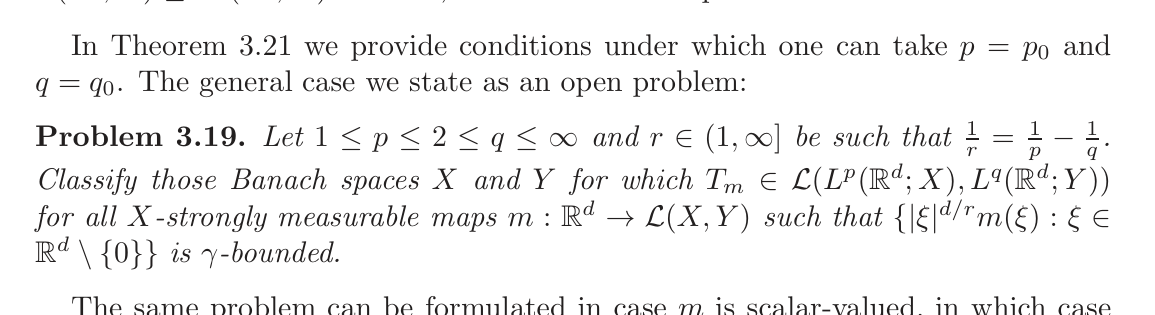
\includegraphics[width=0.95\linewidth]{figures/problem_3_19_crop.png}
\end{center}

This packet consolidates the previous run artifacts for arXiv:1605.09340 into one authoritative packet.  It contains:
\begin{itemize}
\item the complete scalar classification of Problem 3.19;
\item endpoint obstructions for every nonzero Banach pair \(X,Y\);
\item the repaired form of Theorem 3.21 and the proof-gap explanation for its printed \(p=1\) endpoint;
\item the latest interior obstruction and literature map.
\end{itemize}

The status is \emph{partial result, likely valid}.  The packet does not claim a full classification of the remaining interior Banach-valued problem.

\section*{Proof Intuition}

There are two separate phenomena.

First, all endpoint failures are scalar.  A nonzero pair \(X,Y\) contains a rank-one scalar channel: choose \(x^*\in X^*\), \(x_0\in X\), and \(y_0\in Y\), and set
\[
  m(\xi)x=a(\xi)x^*(x)y_0 .
\]
If \(|\xi|^{d/r}a(\xi)\) is bounded, then the corresponding operator family is \(\gamma\)-bounded.  Testing on \(f(t)=h(t)x_0\) reduces the Banach-valued estimate to the scalar multiplier \(a\).  The scalar endpoint failure is the classical strong endpoint failure of the Riesz potential: approximate identities see the kernel singularity \(|x|^{-d/q}\) and produce logarithmic \(L^q\) blowup.  The \(q=\infty\) face follows by duality from the same even Riesz multiplier.

Second, the corrected positive theorem uses a Sobolev--\(\gamma\) bridge.  The source proof factors through
\[
  \dot H_p^{d/p-d/2}(\R^d;X)\hookrightarrow\gamma(\R^d;X),
  \qquad
  \gamma(\R^d;Y)\hookrightarrow \dot H_q^{d/q-d/2}(\R^d;Y).
\]
These embeddings are available in the source paper's non-endpoint type/cotype range and in the sharp \(p\)-convex/\(q\)-concave lattice setting for \(1<p\le2\le q<\infty\).  At \(p=1\) the first embedding would imply a false strong endpoint Sobolev/Riesz estimate.  That is the small but decisive gap in the printed endpoint of Theorem 3.21.

\section*{The Scalar Classification}

\begin{theorem}[Scalar form of Problem 3.19]\label{thm:scalar}
Let \(d\ge1\).  In the scalar case \(X=Y=\C\), the property in Problem 3.19 holds for the admissible exponents \(1\le p\le2\le q\le\infty\), \(r\in(1,\infty]\), \(1/r=1/p-1/q\), if and only if
\[
  1<p\le2\le q<\infty .
\]
\end{theorem}

\begin{proof}
If \(1<p\le2\le q<\infty\), scalar \(\gamma\)-boundedness is just uniform boundedness.  Hence
\[
  |m(\xi)|\le C|\xi|^{-d/r}.
\]
For \(r<\infty\), this implies \(m\in L^{r,\infty}(\R^d)\), and the scalar H\"ormander multiplier theorem quoted in the source paper gives \(T_m:L^p(\R^d)\to L^q(\R^d)\).  If \(r=\infty\), then \(p=q=2\), and the conclusion follows from Plancherel.

Now let \(p=1\), \(2\le q<\infty\), and \(r=q'\).  Put
\[
  a_q(\xi)=|\xi|^{-d/q'}\qquad(\xi\ne0),
\]
with any value assigned at \(\xi=0\).  Then \(|\xi|^{d/q'}a_q(\xi)=1\) for \(\xi\ne0\).  The inverse Fourier transform of \(a_q\) is a nonzero constant multiple of
\[
  K_q(x)=|x|^{-d/q}.
\]
Let \(\eta\in C_c^\infty(\R^d)\) be nonnegative, supported in the unit ball, and satisfy \(\int\eta=1\).  Set \(\eta_\varepsilon(x)=\varepsilon^{-d}\eta(x/\varepsilon)\).  For \(2\varepsilon\le |x|\le1/2\) and \(y\in\supp(\eta_\varepsilon)\), one has \(|x-y|\simeq |x|\).  Therefore
\[
  |T_{a_q}\eta_\varepsilon(x)|\ge c|x|^{-d/q}
\]
on this annulus, and hence
\[
  \|T_{a_q}\eta_\varepsilon\|_q^q
  \ge c^q\int_{2\varepsilon\le |x|\le1/2}|x|^{-d}\,dx
  \simeq \log(1/\varepsilon)\to\infty .
\]
But \(\|\eta_\varepsilon\|_1=1\).  Thus \(T_{a_q}\) is not bounded \(L^1\to L^q\).

Finally let \(1<p\le2\) and \(q=\infty\).  Then \(r=p\).  If the scalar property held for this pair, it would hold for the real even multiplier
\[
  a_p(\xi)=|\xi|^{-d/p}.
\]
For Schwartz \(f,g\), Fourier-side pairing gives
\[
  \langle T_{a_p}f,g\rangle=\langle f,T_{a_p}g\rangle .
\]
Boundedness \(T_{a_p}:L^p\to L^\infty\) would imply
\[
  |\langle f,T_{a_p}g\rangle|
  \le C\|f\|_p\|g\|_1 .
\]
Taking the supremum over \(\|f\|_p\le1\) yields \(T_{a_p}:L^1\to L^{p'}\), contradicting the \(p=1\) endpoint failure just proved with target exponent \(p'\).  This proves the scalar classification.
\end{proof}

\section*{Endpoint Obstructions for Nonzero Banach Pairs}

\begin{theorem}[Endpoint obstruction for all nonzero pairs]\label{thm:endpoints}
Let \(d\ge1\), and let \(X,Y\) be nonzero Banach spaces.
\begin{enumerate}
\item If \(p=1\), \(2\le q<\infty\), and \(r=q'\), then Problem 3.19 fails for the pair \(X,Y\).
\item If \(1<p\le2\), \(q=\infty\), and \(r=p\), then Problem 3.19 fails for the pair \(X,Y\).
\end{enumerate}
\end{theorem}

\begin{proof}
Choose \(x_0\in X\), \(x^*\in X^*\), \(y_0\in Y\), and \(y^*\in Y^*\) such that
\[
  x^*(x_0)=1,\qquad y_0\ne0,\qquad y^*(y_0)=1.
\]

For \(p=1\), \(2\le q<\infty\), let \(a_q(\xi)=|\xi|^{-d/q'}\) and define
\[
  m(\xi)x=a_q(\xi)x^*(x)y_0.
\]
The weighted family is \(\gamma\)-bounded.  Indeed, for finite choices \(\xi_j\ne0\), \(u_j\in X\), and \(\lambda_j=|\xi_j|^{d/q'}a_q(\xi_j)\), one has \(|\lambda_j|=1\), and
\begin{align*}
\Big(\mathbb E\Big\|\sum_j\gamma_j\lambda_jx^*(u_j)y_0\Big\|_Y^2\Big)^{1/2}
&\le \|y_0\|\Big(\sum_j |x^*(u_j)|^2\Big)^{1/2}\\
&\le \|y_0\|\,\|x^*\|
   \Big(\mathbb E\Big\|\sum_j\gamma_j u_j\Big\|_X^2\Big)^{1/2}.
\end{align*}
Testing on \(f_\varepsilon=\eta_\varepsilon x_0\) gives
\[
  T_m f_\varepsilon=(T_{a_q}\eta_\varepsilon)y_0.
\]
By Theorem \ref{thm:scalar}, the \(L^q(Y)\)-norms diverge while \(\|f_\varepsilon\|_{L^1(X)}\) remains bounded.  Thus the \(p=1\) endpoint fails.

For \(1<p\le2\), \(q=\infty\), define
\[
  m_p(\xi)x=|\xi|^{-d/p}x^*(x)y_0 .
\]
The same rank-one estimate shows that \(\{|\xi|^{d/p}m_p(\xi):\xi\ne0\}\) is \(\gamma\)-bounded.  If \(T_{m_p}:L^p(\R^d;X)\to L^\infty(\R^d;Y)\) were bounded, then testing on \(fx_0\) and applying \(y^*\) would imply the scalar boundedness
\[
  T_{a_p}:L^p(\R^d)\to L^\infty(\R^d),
  \qquad a_p(\xi)=|\xi|^{-d/p},
\]
contradicting the scalar \(q=\infty\) failure in Theorem \ref{thm:scalar}.  Hence this endpoint fails for every nonzero pair \(X,Y\).
\end{proof}

\begin{corollary}[Remaining exponent core]\label{cor:core}
For nonzero \(X,Y\), the only exponent range in Problem 3.19 where a nontrivial positive classification can remain is
\[
  1<p\le2\le q<\infty.
\]
The formal corner \(p=1,q=\infty\) is not admissible in Problem 3.19, since it would force \(r=1\), while the problem assumes \(r\in(1,\infty]\).
\end{corollary}

\section*{Theorem 3.21: Printed Endpoint Conflict and Repair}

The source paper's Theorem 3.21 is printed for
\[
  p\in[1,2],\qquad q\in[2,\infty),
\]
and says that, under \(p\)-convex/\(q\)-concave lattice hypotheses, the same weighted \(\gamma\)-boundedness assumption implies \(T_m:L^p(\R^d;X)\to L^q(\R^d;Y)\).

\begin{center}
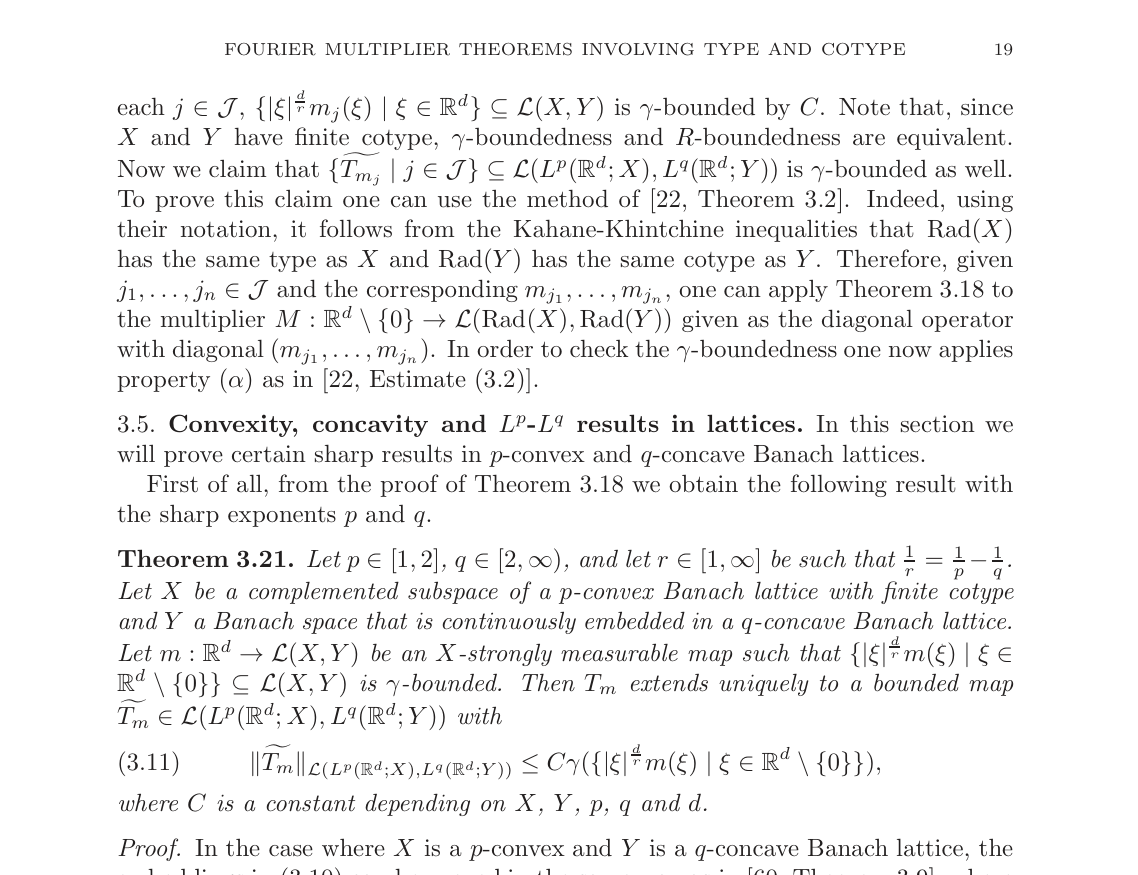
\includegraphics[width=0.95\linewidth]{figures/theorem_3_21_crop.png}
\end{center}

The literal \(p=1\) endpoint conflicts with Theorem \ref{thm:endpoints}: take \(X=Y=\C\).  More concretely, at \(p=1,q=2,r=2\), the scalar multiplier
\[
  m(\xi)=\mathbf 1_{\{|\xi|\ge1\}}|\xi|^{-d/2}
\]
has bounded weighted set \(\{|\xi|^{d/2}m(\xi):\xi\ne0\}\), but approximate identities and Plancherel give logarithmic \(L^2\)-blowup.  The high-frequency cutoff merely removes any possible concern about the multiplier at \(\xi=0\); the endpoint obstruction is the same Riesz singularity.

The proof passage for Theorem 3.21 says that the embeddings used in Theorem 3.18 can be proved for \(p\)-convex and \(q\)-concave lattices and then imports the proof of Theorem 3.18.

\begin{center}
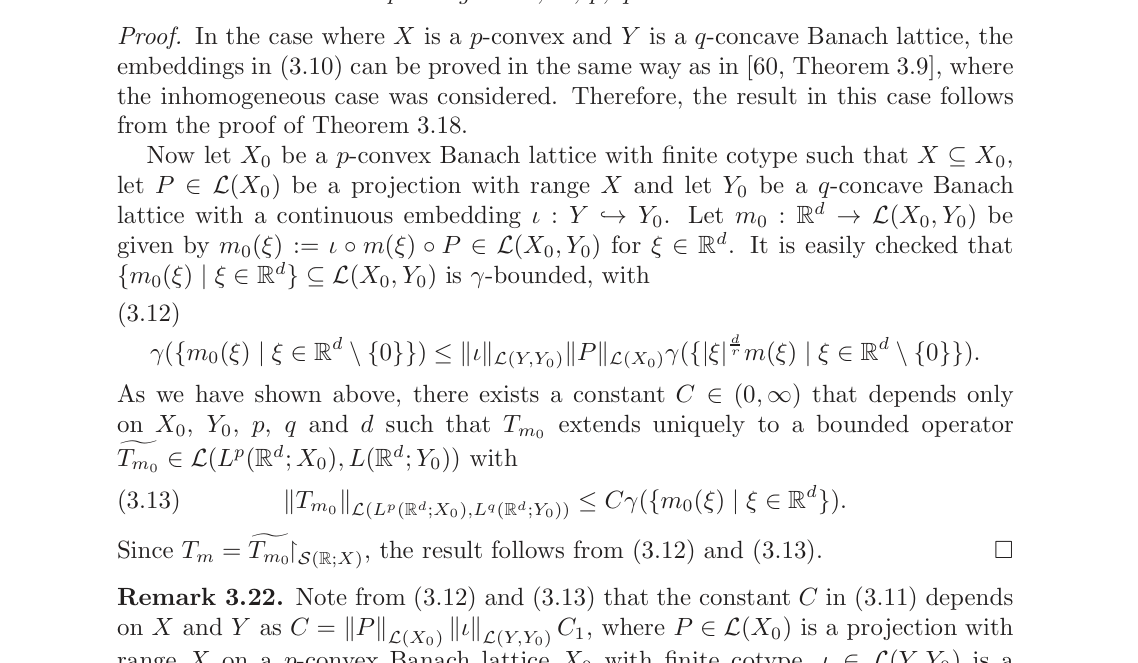
\includegraphics[width=0.95\linewidth]{figures/theorem_3_21_proof_crop.png}
\end{center}

At \(p=1\), that embedding would imply a false strong endpoint Sobolev/Riesz estimate.  For \(1<p\le2\), the same argument is valid.

\begin{theorem}[Repaired Theorem 3.21]\label{thm:repair}
Let \(1<p\le2\), \(2\le q<\infty\), and let \(r\in(1,\infty]\) satisfy
\[
  \frac1r=\frac1p-\frac1q.
\]
Let \(X\) be a complemented subspace of a \(p\)-convex Banach lattice with finite cotype, and let \(Y\) be a Banach space that embeds continuously into a \(q\)-concave Banach lattice.  If \(m:\R^d\setminus\{0\}\to\cL(X,Y)\) is \(X\)-strongly measurable and
\[
  \{|\xi|^{d/r}m(\xi):\xi\ne0\}
\]
is \(\gamma\)-bounded, then \(T_m\) extends uniquely to a bounded operator
\[
  T_m:L^p(\R^d;X)\to L^q(\R^d;Y),
\]
with norm bounded by a constant depending on \(X,Y,p,q,d\) times the displayed \(\gamma\)-bound.
\end{theorem}

\begin{proof}
In the lattice case the homogeneous embedding input is
\[
  \dot H_p^{d/p-d/2}(\R^d;X)\hookrightarrow \gamma(\R^d;X),
  \qquad
  \gamma(\R^d;Y)\hookrightarrow \dot H_q^{d/q-d/2}(\R^d;Y).
\]
For \(1<p\le2\le q<\infty\), this is exactly the non-endpoint \(p\)-convex/\(q\)-concave embedding input cited by the source proof, based on Veraar's embedding results for \(\gamma\)-spaces and the Kalton--van Neerven--Veraar--Weis Besov-to-\(\gamma\) embeddings.

Set
\[
  m_1(\xi)=|\xi|^{d/2-d/p},\qquad
  m_2(\xi)=|\xi|^{d/r}m(\xi)m_1(\xi).
\]
For \(f\in\mathcal S(\R^d;X)\), the source proof gives
\begin{align*}
\|T_m f\|_{L^q(\R^d;Y)}
&= \|T_{m_2}f\|_{\dot H_q^{d/q-d/2}(\R^d;Y)}\\
&\le C\|T_{m_2}f\|_{\gamma(\R^d;Y)}\\
&\le C\,\gamma(\{|\xi|^{d/r}m(\xi):\xi\ne0\})
       \|m_1\widehat f\|_{\gamma(\R^d;X)}\\
&\le C\,\gamma(\{|\xi|^{d/r}m(\xi):\xi\ne0\})
       \|T_{m_1}f\|_{\dot H_p^{d/p-d/2}(\R^d;X)}\\
&= C\,\gamma(\{|\xi|^{d/r}m(\xi):\xi\ne0\})\,\|f\|_{L^p(\R^d;X)}.
\end{align*}
The middle estimate is the \(\gamma\)-multiplier theorem.  Density of Schwartz functions in \(L^p\) gives the bounded extension.

For complemented subspaces and embedded targets, let \(X\subseteq X_0\) be the range of a bounded projection \(P:X_0\to X\), where \(X_0\) is a \(p\)-convex Banach lattice with finite cotype, and let \(\iota:Y\to Y_0\) be a continuous embedding into a \(q\)-concave Banach lattice.  Apply the lattice case to
\[
  m_0(\xi)=\iota\,m(\xi)P\in\cL(X_0,Y_0).
\]
The weighted family for \(m_0\) has \(\gamma\)-bound at most
\[
  \|\iota\|\,\|P\|\,
  \gamma(\{|\xi|^{d/r}m(\xi):\xi\ne0\}).
\]
Restricting back to \(X\) proves the stated theorem.
\end{proof}

\begin{corollary}
The \(p=1\) endpoint in the printed Theorem 3.21 cannot be rescued for nonzero spaces under only the stated weighted \(\gamma\)-boundedness hypothesis.  The sharp corrected strong range is \(1<p\le2\), \(2\le q<\infty\).
\end{corollary}

\section*{Interior Range: What Remains Open}

After Corollary \ref{cor:core}, the possible nontrivial range for Problem 3.19 is
\[
  1<p\le2\le q<\infty.
\]
The source paper proves a large sufficient theorem: if \(X\) has type \(p_0\in(1,2]\), \(Y\) has cotype \(q_0\in[2,\infty)\), and
\[
  1<p<p_0,\qquad q_0<q<\infty,
\]
with the Hilbert endpoint allowances when \(p_0=2\) or \(q_0=2\), then Problem 3.19 has a positive answer.  The repaired Theorem \ref{thm:repair} gives a sharp class in the lattice setting.

The best abstract reduction is the following: a full positive theorem in the expected type/cotype form would follow from the endpoint Bessel--\(\gamma\) embeddings
\[
  \dot H_p^{d/p-d/2}(\R^d;X)\hookrightarrow\gamma(\R^d;X),
  \qquad
  \gamma(\R^d;Y)\hookrightarrow\dot H_q^{d/q-d/2}(\R^d;Y).
\]
The decisive known theorem of Kalton--van Neerven--Veraar--Weis characterizes type and cotype by the adjacent Besov embeddings
\[
  B_{p,p}^{d(1/p-1/2)}(\R^d;X)\hookrightarrow \gamma(L^2(\R^d),X)
\]
and
\[
  \gamma(L^2(\R^d),Y)\hookrightarrow B_{q,q}^{d(1/q-1/2)}(\R^d;Y).
\]
For \(p<2\), the Besov space \(B_{p,p}^s\) is smaller than the Bessel/Triebel--Lizorkin space \(H_p^s=F_{p,2}^s\) needed in the multiplier proof.  Dually, the cotype conclusion lands in the wrong summability scale for the target Bessel embedding.  This is the main remaining summability gap.

The Rozendaal--Veraar Besov companion paper proves optimal type/cotype exponents in the Besov scale and derives an \(L^p\to L^q\) theorem under the dyadic condition
\[
  \big(2^{kd/r}\gamma(\{m(\xi):\xi\in J_k\})\big)_{k\in\mathbb Z}\in\ell^1(\mathbb Z).
\]
This condition is stronger than Problem 3.19's uniform weighted gamma-bound, which only gives a bounded dyadic sequence.

Dominguez--Veraar later developed vector-valued Pitt inequalities.  Their endpoint theorem gives the right Bochner estimate in key cases, for example
\[
  \big\||\xi|^{-d(1/p-1/2)}\widehat f(\xi)\big\|_{L^2(\R^d;X)}
  \lesssim \|f\|_{L^p(\R^d;X)}
\]
when \(X\) has suitable Fourier type.  This is not the same as the gamma-radonifying embedding above; passing from Bochner \(L^2(X)\) to \(\gamma(L^2,X)\) requires additional square-function geometry, such as the Hilbert or lattice structures already covered.

Finally, the source paper's Schur multiplier problem asks whether a Schatten-class endpoint \(1/r=|1/a-1/2|\) can be reached.  The authors note that a negative answer would imply failure of
\[
  H_a^{1/a-1/2}(\R;S^a)\to\gamma(\R;S^a),\qquad 1<a<2.
\]
This is the same Bessel--\(\gamma\) endpoint obstruction.  Modern Littlewood--Paley--Stein and Lusin type/cotype results are adjacent to this issue, but the literature search did not locate a theorem converting those square-function estimates into the global radonifying embedding required here.

\section*{Verification Notes}

\begin{itemize}
\item The scalar positive range uses only the scalar weak-\(L^r\) H\"ormander theorem quoted in the source paper.  The case \(r=\infty\) is \(p=q=2\) and follows from Plancherel.
\item The scalar \(p=1\) failure is the standard endpoint Riesz-potential failure; the logarithmic divergence is localized on \(2\varepsilon\le |x|\le1/2\).
\item The \(q=\infty\) failure uses Schwartz-pairing duality and does not identify the dual of \(L^\infty\).
\item The rank-one reduction proves that the endpoint failures are not artifacts of \(X=Y=\C\); they occur for every nonzero pair.
\item The Theorem 3.21 repair deletes exactly the endpoint contradicted by the rank-one obstruction.  For \(1<p\le2\), the proof is the source paper's Sobolev--\(\gamma\) multiplier argument.
\item The interior material is recorded as an obstruction/reduction, not as a proof of the full classification.
\end{itemize}

\section*{Literature and Duplicate Checks}

The run indexes were checked for \texttt{1605.09340}, Problem 3.19, Theorem 3.21, scalar classification, endpoint repair, proof gap, Pitt inequality, type/cotype, Besov multiplier, and Sobolev--\(\gamma\) phrases.  The separate earlier artifacts have been consolidated into this packet.

External literature checks covered the source paper, the Besov companion arXiv:1606.03272, Kalton--van Neerven--Veraar--Weis arXiv:math/0610620, Dominguez--Veraar arXiv:1904.07930, and modern Littlewood--Paley--Stein/Lusin type papers including arXiv:2105.12175 and arXiv:2401.13932.  No full later classification of Problem 3.19 or erratum for Theorem 3.21 was found in this search.

\section*{Superseded Run Artifacts}

This packet supersedes the following previous run artifacts:
\begin{itemize}
\item \texttt{solutions/partial/1605.09340\_scalar\_endpoint\_multiplier\_failure/}
\item \texttt{solutions/partial/1605.09340\_theorem\_3\_21\_endpoint\_repair/}
\item \texttt{solutions/partial/1605.09340\_problem\_3\_19\_endpoint\_core\_reduction/}
\item \texttt{proof\_gaps/1605.09340\_theorem\_3\_21\_scalar\_endpoint\_conflict/}
\item \texttt{attempts/1605.09340\_problem\_3\_19\_interior\_literature\_full\_push.md}
\end{itemize}

\section*{References}

\begin{thebibliography}{99}

\bibitem{RV}
J. Rozendaal and M. Veraar, \emph{Fourier multiplier theorems involving type and cotype}, arXiv:1605.09340; J. Fourier Anal. Appl. 24 (2018), no. 2, 583--619.

\bibitem{RVB}
J. Rozendaal and M. Veraar, \emph{Fourier multiplier theorems on Besov spaces under type and cotype conditions}, arXiv:1606.03272; Banach J. Math. Anal. 11 (2017), no. 4, 713--743.

\bibitem{KNVW}
N. J. Kalton, J. van Neerven, M. Veraar, and L. Weis, \emph{Embedding vector-valued Besov spaces into spaces of \(\gamma\)-radonifying operators}, Math. Nachr. 281 (2008), no. 2, 238--252; arXiv:math/0610620.

\bibitem{Veraar}
M. Veraar, \emph{Embedding results for \(\gamma\)-spaces}, in \emph{Recent trends in analysis}, Theta Foundation, 2013, 209--219.

\bibitem{DV}
O. Dominguez and M. Veraar, \emph{Extensions of the vector-valued Hausdorff--Young inequalities}, J. Fourier Anal. Appl. 25 (2019), 3793--3845; arXiv:1904.07930.

\bibitem{Xu}
Q. Xu, \emph{Holomorphic functional calculus and vector-valued Littlewood--Paley--Stein theory for semigroups}, arXiv:2105.12175.

\bibitem{HXZ}
G. Hong, Z. Xu, and H. Zhang, \emph{Best constants in the vector-valued Littlewood--Paley--Stein theory}, arXiv:2401.13932.

\bibitem{Hormander}
L. H\"ormander, \emph{Estimates for translation invariant operators in \(L^p\) spaces}, Acta Math. 104 (1960), 93--140.

\bibitem{Grafakos}
L. Grafakos, \emph{Classical Fourier Analysis}, Graduate Texts in Mathematics 249, Springer, second edition, 2008.

\bibitem{Beckner}
W. Beckner, \emph{Pitt's inequality with sharp convolution estimates}, Proc. Amer. Math. Soc. 136 (2008), no. 5, 1871--1885.

\bibitem{BenedettoHeinig}
J. J. Benedetto and H. P. Heinig, \emph{Weighted Fourier inequalities: new proofs and generalizations}, J. Fourier Anal. Appl. 9 (2003), no. 1, 1--37.

\end{thebibliography}

\section*{Human Review Recommendation}

Review the Riesz-potential endpoint proof, the rank-one \(\gamma\)-boundedness estimate, and the use of the \(p>1\) Sobolev--\(\gamma\) embedding in the repaired theorem.  If these pass, this single packet should replace the earlier separate scalar, proof-gap, repair, endpoint-core, and interior-attempt records.  The remaining interior classification should stay marked open/partial unless a proof or counterexample for the endpoint Bessel--\(\gamma\) mechanism is found.

\begin{reviewnote}
This is a consolidation packet.  It intentionally preserves the full mathematical content of the earlier packets while leaving only one active durable record for arXiv:1605.09340 in the run indexes.
\end{reviewnote}

\end{document}
